% Converted from reference/DB4OTutorial (MadCap Flare, Java target)

\chapter{Update Concept}
\label{tut:update-concept}

How does updating objects work with db4o? Similar to the activation depth, db4o uses an update depth. When we store an object again, db4o only updates the objects up to the given update-depth. This prevents db4o from traversing the whole object graph in order to store the changes.

\begin{center}
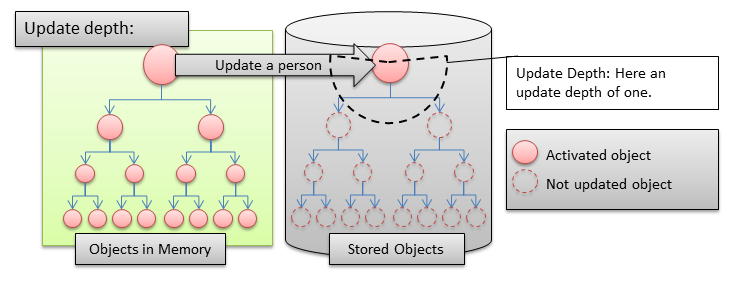
\includegraphics[width=\maxwidth]{images/tut-update-depth.png}
\end{center}
\section{Updating in Action}
\label{tut:update-concept:updatedepthinaction}

Let's see db4o's update strategy in action. We store a driver with his cars and his most loved car.

\begin{lstlisting}
public class Car {
    private String carName;

    public Car(String carName) {
        this.carName = carName;
    }

    public String getCarName() {
        return carName;
    }

    public void setCarName(String carName) {
        this.carName = carName;
    }

    @Override
    public String toString() {
        return "Car{" +
                "carName='" + carName + '\'' +
                '}';
    }
}
\end{lstlisting}

{\small\itshape Car.java: Domain model for cars\par}
\medskip

\begin{lstlisting}
public class Driver {
    private String name;
    private final List<Car> ownedCars = new ArrayList<Car>();
    private Car mostLovedCar;

    public Driver(String name) {
        this.name = name;
    }

    public Driver(String name, Car mostLovedCar) {
        this.name = name;
        this.mostLovedCar = mostLovedCar;
    }

    public void setName(String name) {
        this.name = name;
    }

    public String getName() {
        return name;
    }

    public Car getMostLovedCar() {
        return mostLovedCar;
    }

    public Iterable<Car> getOwnedCars() {
        return ownedCars;
    }

    public boolean addOwnedCar(Car car) {
        return ownedCars.add(car);
    }
}
\end{lstlisting}

{\small\itshape Driver.java: Domain model for drivers\par}
\medskip

\begin{lstlisting}
Car beetle = new Car("VW Beetle");
Car ferrari = new Car("Ferrari");

Driver driver = new Driver("John", ferrari);
driver.addOwnedCar(beetle);
driver.addOwnedCar(ferrari);

container.store(driver);
\end{lstlisting}

{\small\itshape UpdateConcept.java: Store a driver and his cars\par}
\medskip

After that we update the driver, change the name of his most loved car and add another car to his collection. Then we update the car in the database.

\begin{lstlisting}
Driver driver = queryForDriver(container);
driver.setName("Johannes");
driver.getMostLovedCar().setCarName("Red Ferrari");
driver.addOwnedCar(new Car("Fiat Punto"));
container.store(driver);
\end{lstlisting}

{\small\itshape UpdateConcept.java: Update the driver and his cars\par}
\medskip

Then we close the database, reopen it and check if the objects have been updated. Unfortunately only the car itself has been updated. That's because db4o by default uses an update-depth of one. That means only the object we pass to the store-method is updated. All referenced objects are not updated. In our case that means that the referenced car and the referenced list of cars isn't updated.

\begin{lstlisting}
Driver driver = queryForDriver(container);
// Is updated
System.out.println(driver.getName());
// Isn't updated at all
System.out.println(driver.getMostLovedCar().getCarName());
// Also the owned car list isn't updated
for (Car car : driver.getOwnedCars()) {
    System.out.println(car);
}
\end{lstlisting}

{\small\itshape UpdateConcept.java: Check the updated objects\par}
\medskip

\section{Deal with Updates}
\label{tut:update-concept:dealwithit}

We've seen that by default only the object passed to the store method is updated. That means we need a strategy to deal with this.

\subsection*{Explicitly Storing Every Changed Object}

One way to deal with this is to store every changed object. In our case that would be the driver, the most loved car and the list of owed cars. However in practice this strategy needs too much effort.

\begin{lstlisting}
container.store(driver);
container.store(driver.getMostLovedCar());
container.store(driver.getOwnedCars());
\end{lstlisting}

{\small\itshape UpdateConcept.java: Update everything explicitly\par}
\medskip

\subsection*{Change the Activation Depth}

A simple strategy is to increase the update depth, for example increase the depth to two. This is quite a reasonable update-depth, especially since it will update collections of an object.

\begin{lstlisting}
EmbeddedConfiguration configuration = Db4oEmbedded.newConfiguration();
configuration.common().updateDepth(2);
\end{lstlisting}

{\small\itshape UpdateConcept.java: Increase the update depth to 2\par}
\medskip

We can control the update-depth also per class:

\begin{lstlisting}
EmbeddedConfiguration configuration = Db4oEmbedded.newConfiguration();
// Update all referenced objects for the Driver class
configuration.common().objectClass(Driver.class).cascadeOnUpdate(true);
\end{lstlisting}

{\small\itshape UpdateConcept.java: More update options\par}
\medskip

\subsection*{Transparent Persistence}

The last and most elaborate option is to use transparent persistence. In that case db4o manages all updates for us. We just can change objects and db4o will track all changes for us. To get transparent persistence we need to enhance our classes at compile time. Read \hyperref[tut:transparentpersistence]{this section of the tutorial} (p.~\pageref{tut:transparentpersistence}) where we use transparent persistence.

